\documentclass[crop,tikz]{standalone}
\usetikzlibrary{backgrounds}
\colorlet{blue}{cyan}
\tikzset{
  inverted/.style = {
    color=white,
    background rectangle/.style={fill},
    show background rectangle
  }
}

\usepackage{pgfplots}
\pgfplotsset{compat=1.16}

% rainbow line
\pgfdeclareverticalshading{rainbow}{100bp}
{color(0bp)=(red); color(25bp)=(red); color(35bp)=(yellow);
color(45bp)=(green); color(55bp)=(cyan); color(65bp)=(blue);
color(75bp)=(violet); color(100bp)=(violet)}

\begin{document}
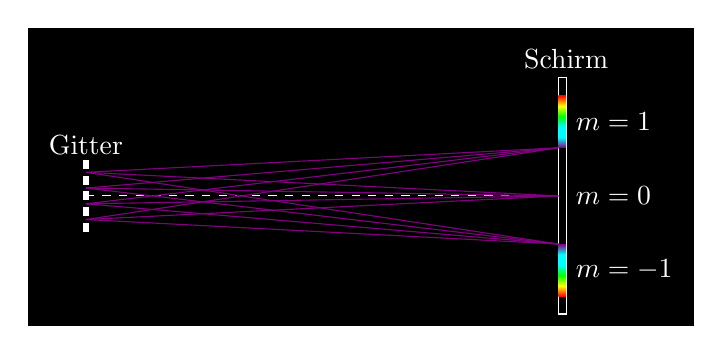
\begin{tikzpicture}[inverted,inverted]
  \pgfmathsetmacro{\projectionheight}{3}
  \pgfmathsetmacro{\projectionwidth}{0.1}
  \pgfmathsetmacro{\gratingwidth}{0.06}
  \pgfmathsetmacro{\gratingheight}{0.4}
  \pgfmathsetmacro{\wavelengthred}{780} % nm
  \pgfmathsetmacro{\wavelengthviolet}{380} % nm
  \pgfmathsetmacro{\gratingconstant}{3750}
  \pgfmathsetmacro{\distance}{6}
  \pgfmathsetmacro{\ared}{\distance*tan(asin(\wavelengthred/\gratingconstant))}
  \pgfmathsetmacro{\aviolet}{\distance*tan(asin(\wavelengthviolet/\gratingconstant))}
  % central line
  \draw[dashed] (0,0) -- (\distance,0);
  % grating
  \foreach \Y in { -0.4,-0.2,...,0.4 } {%
    \draw[fill] ({-\gratingwidth/2},\Y - 0.05) rectangle ({\gratingwidth/2},\Y + 0.05);
  };
  \node[above] at (0,\gratingheight) {Gitter};
  % projection
  \draw[] (\distance,{-\projectionheight/2}) rectangle ({\distance+\projectionwidth},{\projectionheight/2}) node[above,white] {Schirm};
  \shade[shading=rainbow,shading angle=180] (\distance,{\aviolet}) rectangle ({\distance+\projectionwidth},{\ared});
  \shade[shading=rainbow,shading angle=0] (\distance,{-\aviolet}) rectangle ({\distance+\projectionwidth},{-\ared});
  % rays
  \foreach \Y in {-0.3,-0.1,...,0.3} {
    \draw[violet] (0,\Y) -- ({\distance},{\aviolet});
    \draw[violet] (0,\Y) -- ({\distance},0);
    \draw[violet] (0,\Y) -- ({\distance},{-\aviolet});
  };
  % labels
  \node[right] at ({\distance+\projectionwidth},0) {$m=0$};
  \node[right] at ({\distance+\projectionwidth},{(\ared+\aviolet)/2}) {$m=1$};
  \node[right] at ({\distance+\projectionwidth},{-(\ared+\aviolet)/2}) {$m=-1$};
\end{tikzpicture}
\end{document}
